\section{Futures} \label{sec:futures}\label{futures}
Consider an outline parallel Arrow combinator:
\begin{code}
someCombinator:: (ArrowChoice arr,
	ArrowParallel arr a b (),
	ArrowParallel arr b c ()) =>
	[arr a b] -> [arr b c] -> arr [a] [c]
someCombinator fs1 fs2 =
	parEvalN () fs1 >>>
	rightRotate >>>
	parEvalN () fs2
\end{code}

In a distributed environment such a combinator first evaluates all |[arr a b]| in parallel, sends the results back to the master node, rotates the input once (in the example we require |ArrowChoice| for this) and then evaluates the |[arr b c]| in parallel to then gather the input once again on the master node.
Such situations arise, \eg in scientific computations when the data distributed across the nodes needs to be transposed. A concrete example is 2D FFT computation \cite{Gorlatch,Berthold2009-fft}.

While the example could be rewritten into a single |parEvalN| call by directly wiring the Arrows together before spawning, it illustrates an important problem. When using a |ArrowParallel| backend that resides on multiple computers, all communication between the nodes is done via the master node, as shown in the Eden trace in Figure~\ref{fig:withoutFutures}. This can become a serious bottleneck
for a larger amount of data and number of processes \citep[as e.g.][showcases]{Berthold2009-fft}.
\begin{figure}[ht]
	\centering
	\includegraphics[width=0.9\textwidth]{images/withoutFutures}
	\caption[without Futures]{Communication between 4 Eden processes without Futures. All communication goes through the master node. Each bar represents one process. Black lines represent communication. Colours: blue $\hat{=}$ idle, green $\hat{=}$ running, red  $\hat{=}$ blocked, yellow $\hat{=}$ suspended.}
	\label{fig:withoutFutures}
% \olcomment{more practical and heavy-weight example! fft (I have the code)?}
% \mbcomment{Depends... Are the communications easy to read in such an example?}
% \mbcomment{Keep the description for the different colours, or link to
%   the EdenTV description in \ref{sec:edentv}}
% \olcomment{ok as is}
% \olcomment{use the fft example (when it works)?}
\end{figure}

This is only a problem in distributed memory (in the scope of this paper) and we should allow nodes to communicate directly with each other. Eden already provides \enquote{remote data} that enable this \cite{AlGo03a,Dieterle2010}.
But as we want code with our DSL to be implementation agnostic, we have to wrap this concept. We do this with the |Future| type class (Fig.~\ref{fig:future}). We require a |conf| parameter here as well, but only so that Haskells type system allows us to have multiple Future implementations imported at once without breaking any dependencies similar to what we did with the |ArrowParallel| type class earlier.
\begin{figure}[h]
\begin{code}
class Future fut a conf | a conf -> fut where
    put :: (Arrow arr) => conf -> arr a (fut a)
    get :: (Arrow arr) => conf -> arr (fut a) a
\end{code}
\caption{Definition of the |Future| type class.}
\label{fig:future}
\end{figure}
Since |RD| is only a type synonym for a communication type that Eden uses internally, we have to use some wrapper classes to fit that definition, though, as Fig.~\ref{fig:RDFuture} shows. %This is due to the same reason we had to introduce a wrapper for |Strategy a| in the GpH Haskell implementation of |ArrowParallel| in Section~\ref{sec:parrows:multicore}.
Technical details are in Appendix, in Section~\ref{app:omitted}.

For GpH and |Par| Monad, we can simply use |BasicFuture|s (Fig.~\ref{fig:BasicFuture}), which are just simple wrappers around the actual data with boiler-plate logic so that the type class is satisfied. This is because the concept of a |Future| does not change anything for shared-memory execution as there are no communication problems to fix. Nevertheless, we require a common interface so the parallel Arrows are portable across backends. The implementation can also be found in Section ~\ref{app:omitted}.

In our communication example we can use this |Future| concept for direct communication between nodes as shown in Fig.~\ref{fig:someCombinatorParallel}.
\begin{figure}[tbh]
\begin{code}
someCombinator :: (ArrowChoice arr, NFData b, NFData c,
	ArrowParallel arr a (fut b) (), 
	ArrowParallel arr (fut b) c (),
	Future fut b ()) =>
	[arr a b] -> [arr b c] -> arr [a] [c]
someCombinator fs1 fs2 =
	parEvalN () (map (>>> put ()) fs1) >>>
	rightRotate >>>
	parEvalN () (map (get () >>>) fs2)
\end{code}
\caption{The mock-up combinator in parallel.}
\label{fig:someCombinatorParallel}
\end{figure}
In a distributed environment, this gives us a communication scheme with messages going through the master node only if it is needed -- similar to what is shown in the trace visualisation in Fig.~\ref{fig:withFutures}. One especially elegant aspect of the definition in Fig.~\ref{fig:future} is that we can specify the type of |Future| to be used per backend with full interoperability between code using different backends, without even requiring to know about the actual type used for communication. We only specify that there has to be a compatible Future and do not care about any specifics as can be seen in Fig.~\ref{fig:someCombinatorParallel}. Note that with our PArrows DSL we can also define default instances |Future fut a ()| for each backend similar to how |ArrowParallel arr a b ()| was defined in Section~\ref{sec:parallel-arrows}. Details can be found in Section~\ref{app:omitted}. \olcomment{Fig. is not really clear. Do Figs with a lot of load? --- fft?}
\begin{figure}[ht]
	\centering
	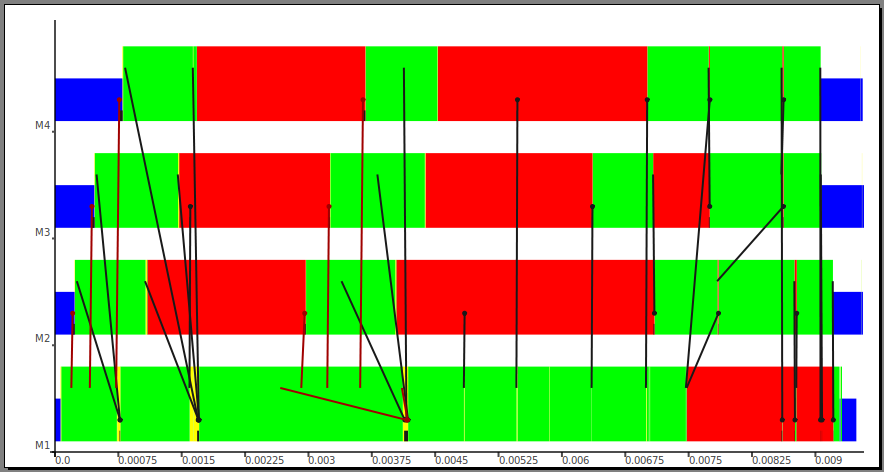
\includegraphics[width=0.9\textwidth]{images/withFutures}
	\caption[with Futures]{Communication between 4 Eden processes with Futures. Other than in Fig.~\ref{fig:withoutFutures}, processes communicate directly (one example message is marked in the Figure) instead of always going through the master node (bottom bar).}
	\label{fig:withFutures}
\end{figure}
